\subsection{Toy Models}

The energy eigenstates and $\set{\ket{0},\ket{1}}$ coefficients for the $H \in \mathbb{R}^2$ Hamiltonian as a function of interaction strength $\lambda$ is shown in figure \cref{fig:res:changing_character}. Despite having two free parameters $C_0,C_1$ they are constrained through normalization.  
\begin{figure}[H]
    \centering
    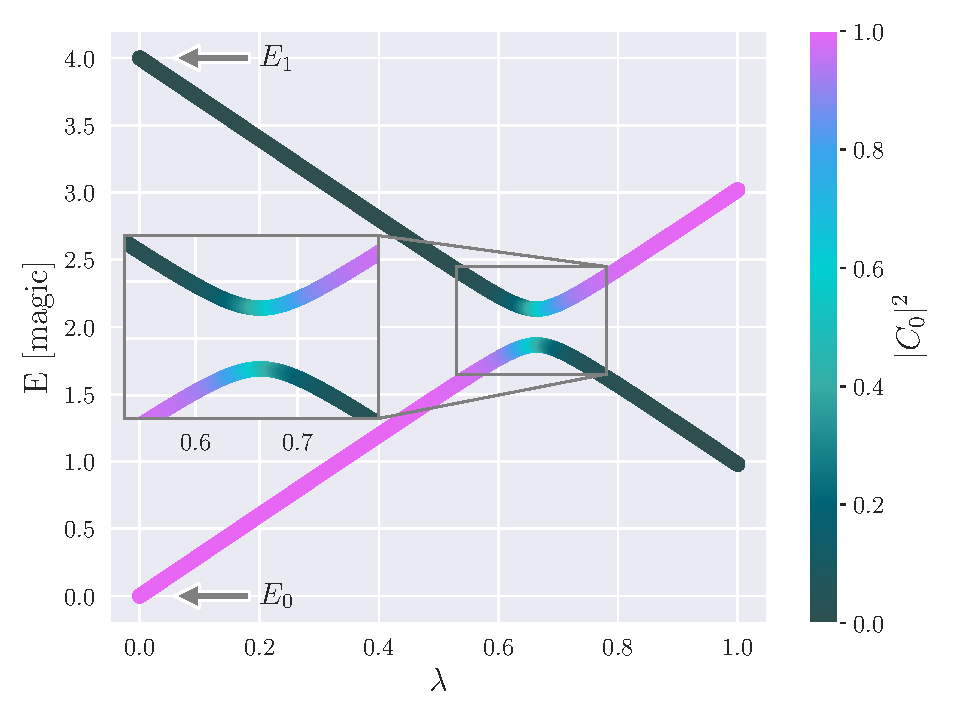
\includegraphics[width=\linewidth]{figs/chaning_character.pdf}
    \caption{Energy eigenstates and coefficients of $2 \times 2$ Hamiltonian when varying the interaction strength $\lambda \in [0,1]$. Calculations done using exact diagonalization.}
    \label[fig]{fig:res:changing_character}
\end{figure}

The entropy of entanglement in the case of the of the Hamiltonian consisting of a interacting and non-interacting between the two states, is presented in Fig. (\ref{fig:entropy}). It is apparent that the entropy of entanglement increases as the connection strength increases. 

\begin{figure}
    \centering
    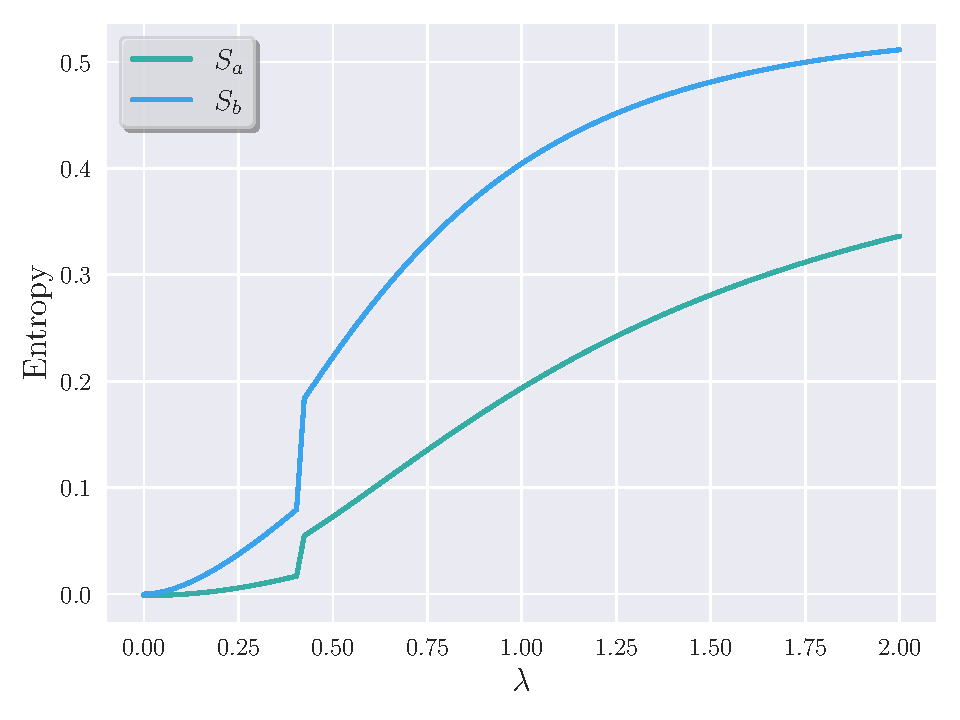
\includegraphics[width=\linewidth]{figs/Entropy.pdf}
    \caption{Caption}
    \label{fig:entropy}
\end{figure}

\subsection{Lipkin Model}
For the Lipkin Model, we initially investigate the $W=0$ case. For the two particles, we apply the VQE where two qbits are required, one for each particle \cref{eq:met:lipkin_N2_dumb}. Additionally, we compare with the HF \cref{eq:theo:hartreefock_lipkin} and RPA \cref{eq:met:lipkin_RPA}. This is shown as a function of $V/\epsilon$ in \cref{fig:res:Lipkin_N2_vary_v}

\begin{figure}[H]
    \centering
    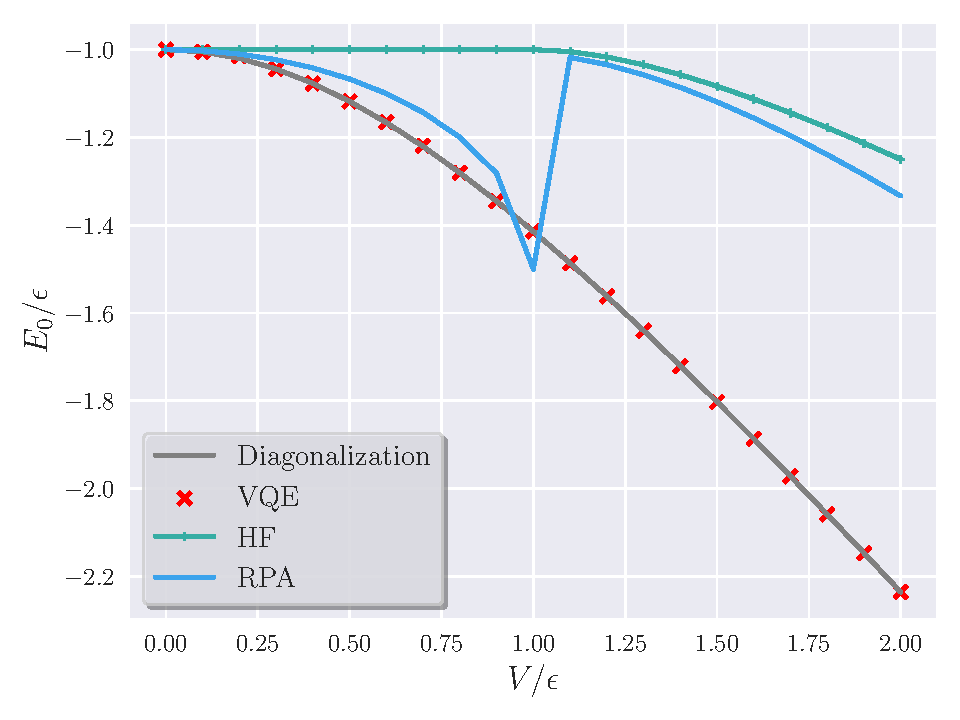
\includegraphics[width=\linewidth]{figs/N2_lipkin_vary_V.pdf}
    \caption{Ground state values for the Lipkin model for $N=2$ particles with $W = 0$ as a function of $V/\epsilon$. Calculations were done using exact diagonalization, VQE with 30 iterations, in addition to closed form HF and RPA expressions.}
    \label[fig]{fig:res:Lipkin_N2_vary_v}
\end{figure}
Moving on to the four particle case, but still keeping $W=0$, we present the energy as a function of $V/\epsilon$ in \cref{fig:res:Lipkin_N4_vary_v}. Here we have used both the $Q=4$ (\cref{eq:met:lipkin_N4_dumb}) and the $Q=2$ (\cref{eq:met:lipkin_N4_smart_hamiltonian}) Hamiltonians. In addition, we also compare with HF and RPA solutions.

\begin{figure}[H]
    \centering
    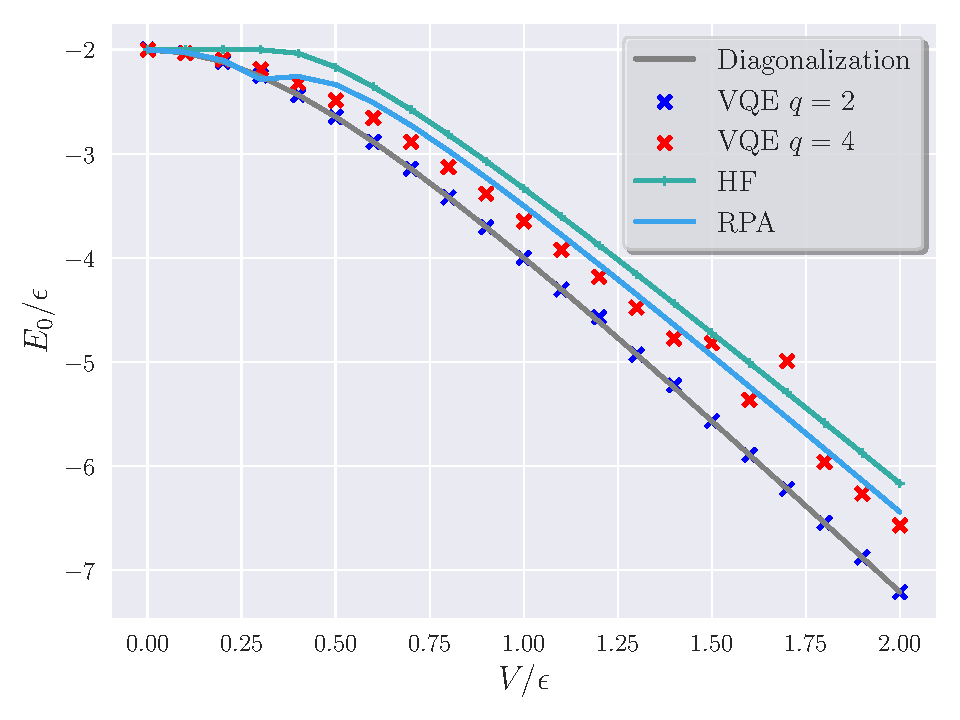
\includegraphics[width=\linewidth]{figs/N4_lipkin_vary_V.pdf}
    \caption{Ground state values for the Lipkin model for $N=4$ particles with $W = 0$ as a function of $V/\epsilon$. Calculations were done using exact diagonalization, VQE for both two (\cref{eq:met:lipkin_N4_smart_hamiltonian}) and four (\cref{eq:met:lipkin_N4_dumb}) qbits, in addition to closed form HF and RPA expressions. The two and four qbit cases were calculated using 300 and 1000 iterations respectively.}
    \label[fig]{fig:res:Lipkin_N4_vary_v}
\end{figure}

Lastly we lift the $W=0$ restriction for four particles and consider the ground state energy as a function of both $V/\epsilon$ and $W/\epsilon$. In \cref{fig:res:lipkin_N4_vw_grid_VQE} we see the relative error from the diagonalization results. Additionally, we benchmark this against the HF and RPA solutions shown in \cref{fig:res:lipkin_N4_vw_grid_HF} and \cref{fig:res:lipkin_N4_vw_grid_RPA} respectively. 
% \begin{figure}[H]
%     \centering
%     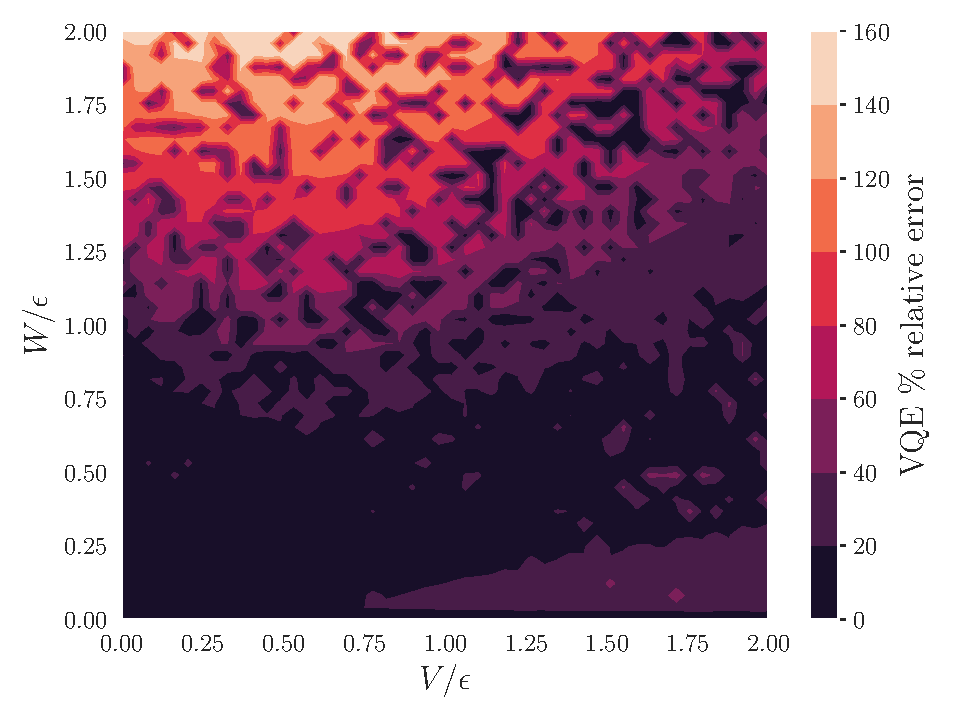
\includegraphics[width=\linewidth]{figs/50pts_vw_grid.pdf}
%     \caption{Relative error in ground state energy for the Lipkin model, using $N=4$ particles as a function of $V/\epsilon$ $W/\epsilon$ and. All energies were calculated using 1000 iterations.}
%     \label[fig]{fig:res:lipkin_N4_vw_grid}
% \end{figure}
\begin{figure}[H]
    \centering
    \begin{subfigure}[b]{\linewidth}
        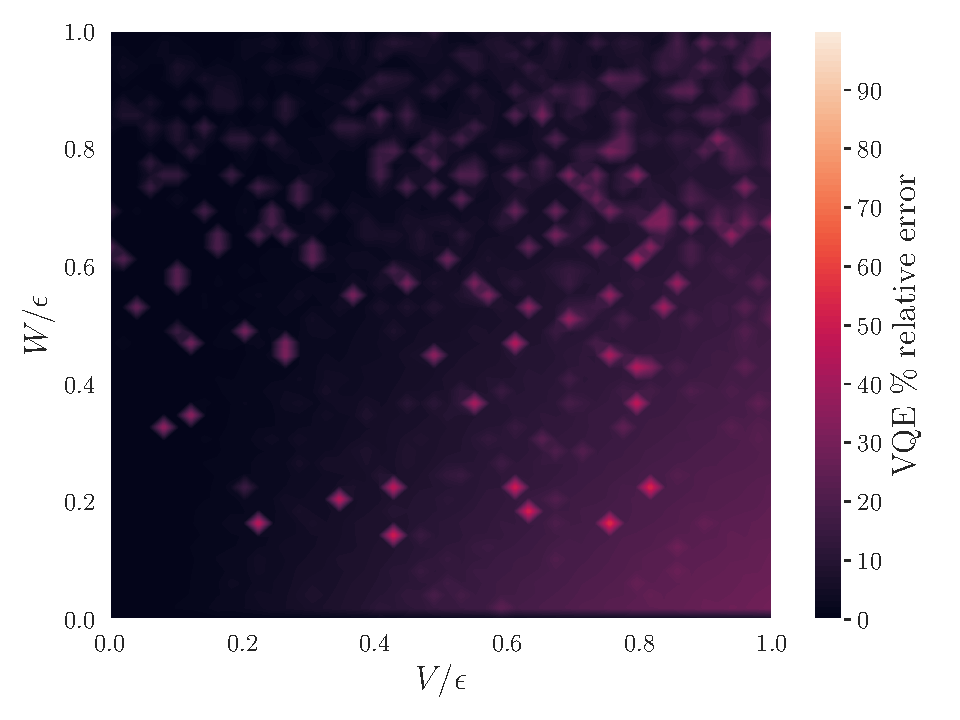
\includegraphics[width=\linewidth]{figs/50pts_vw_grid_VQE.pdf}
        \caption{Variational Quantum Eigensolver. All energies were calculated using 1000 iterations.}
        \label[fig]{fig:res:lipkin_N4_vw_grid_VQE}
    \end{subfigure}
    \begin{subfigure}[b]{\linewidth}
        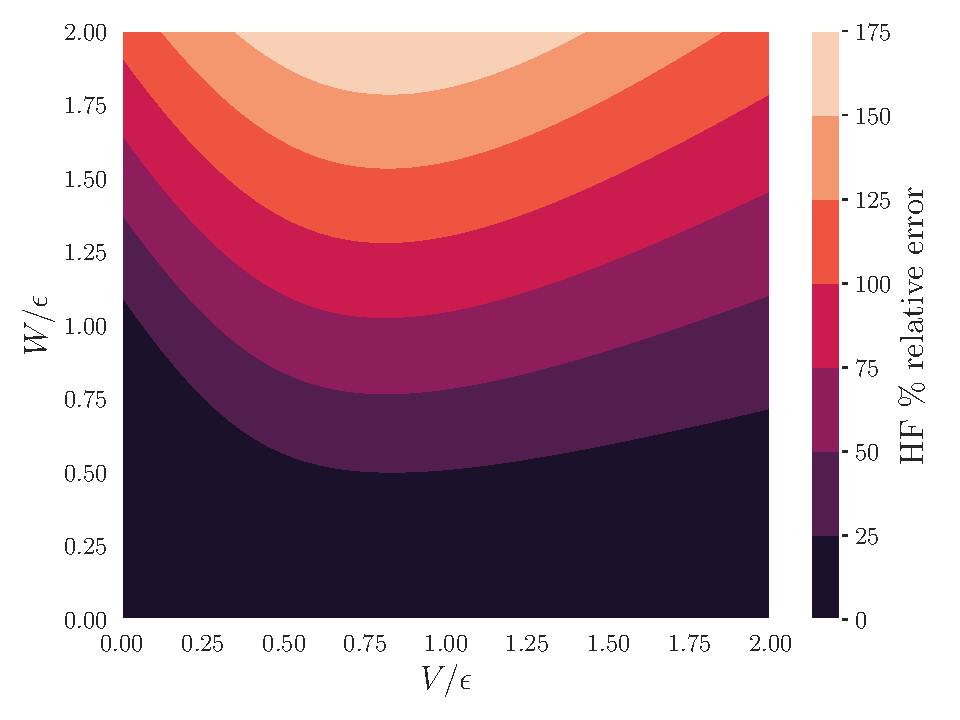
\includegraphics[width=\linewidth]{figs/50pts_vw_grid_HF.pdf}
        \caption{Hartree-Fock, closed form expressions}
        \label[fig]{fig:res:lipkin_N4_vw_grid_HF}
    \end{subfigure}
    \begin{subfigure}[b]{\linewidth}
        \centering
        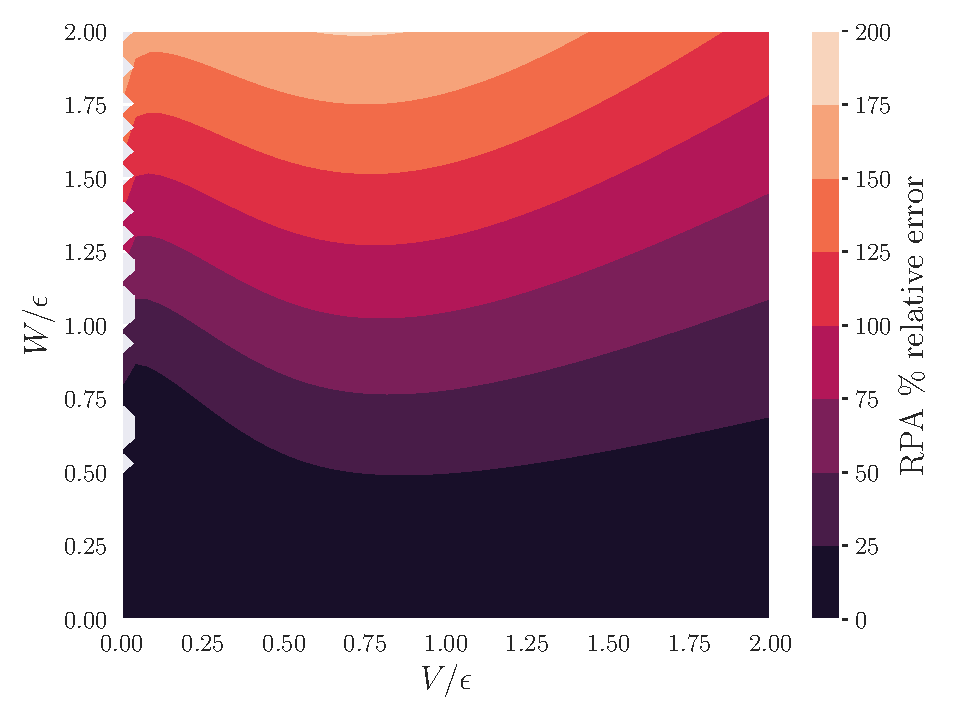
\includegraphics[width=\linewidth]{figs/50pts_vw_grid_RPA.pdf}
        \caption{Random Phase Approximation, closed form expressions}
        \label[fig]{fig:res:lipkin_N4_vw_grid_RPA}
    \end{subfigure}
    \caption{Relative error in ground state energy for the Lipkin model, using $N=4$ particles as a function of $V/\epsilon$ and $W/\epsilon$.}\label[fig]{fig:res:lipkin_N4_vw_grid}
\end{figure}

